\begin{figure}[!htb]
\begin{center}
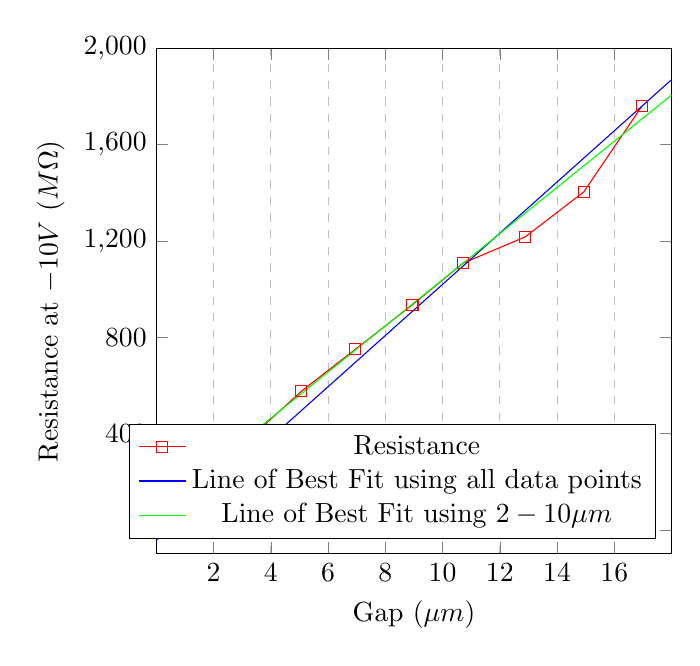
\begin{tikzpicture}

\begin{axis}[
    %title={Temperature dependence of CuSO$_4\cdot$5H$_2$O solubility},
    xlabel={Gap ($\mu m$)},
    ylabel={Resistance at $-10V$ ($M\Omega$)},
    height=8cm,
    width=0.67\textwidth,
    xmin=0, xmax=18,
    ymin=-100, ymax=2000,
    xtick={2, 4, 6, 8, 10,12,14,16},
    ytick={0, 400, 800, 1200, 1600, 2000},
    legend pos=south east,
    xmajorgrids=true,
    grid style=dashed,
]

\addplot[color=red, mark=square]
  coordinates {
    (3.5294, 409.086632)
    (5.0640, 575.542880)
    (6.9493, 749.923132)
    (8.9467, 935.119246)
    (10.719, 1108.230942)
    (12.887, 1217.183218)
    (14.932, 1403.845694)
    (16.966, 1760.563380)
};
  \addlegendentry{Resistance}

\addplot [
  domain=0:18,
  samples=100,
  color=blue,
    ]
      {106.30760633430582*x - 43.05146906783261};
      \addlegendentry{Line of Best Fit using all data points}

\addplot [
  domain=0:18,
  samples=100,
  color=green,
    ]
    {95.89874571698954*x + 80.29228665958908};
  \addlegendentry{Line of Best Fit using $2-10\mu m$}
  % \addlegendentry{Line of Best Fit}


\end{axis}
\end{tikzpicture}

\caption{Plot of Resistance vs TLM Gaps on Substrate A at $250\degree C$ with Line of Best Fit}
\label{fig:results:room_temp_tlms_a_postanneal}
\end{center}
\end{figure}
